%
% Module 2 Chapter 4 Program Documentation
% CSC160-C00: Computer Science I (C++) (Jeffrey Hemmes)
% Author: Ashton Hellwig
% Date: 07 March 2020
%


\documentclass[a4paper, 11pt]{article}
  % Packages
  \usepackage[utf8]{inputenc}         % Encoding
  \usepackage[english]{babel}         % Internationalization
  \usepackage{times}                  % Times New Roman font
  \usepackage{soul}                   % Highlighting
  \usepackage{hyperref}               % Links (internal and external)
  \usepackage{fancyhdr}               % Headers and footers
  \usepackage[dvipsnames]{xcolor}     % Text Colors
  \usepackage{listings}               % Code Snippets
  \usepackage[section]{algorithm}     % For TOC support
  \usepackage{algpseudocode}          % Algorithmic notation environments
  \usepackage{enumitem}               % Ordered lists
  \usepackage{geometry}               % Page layout
  \usepackage{graphicx}               % Image support
  \usepackage{wrapfig}                % Sideways figures (landscape)
  \usepackage{lscape}                 % Sideways figures (landscape)
  \usepackage{rotating}               % Sideways figures (landscape)
  \usepackage{epstopdf}               % Sideways figures (landscape)
  \usepackage[toc, page]{appendix}    % Appendix
  \usepackage{setspace}               % Paragraph and line spacing
  \usepackage{bookmark}               % Required for appendix
  \usepackage{adjustbox}              % Required for appendix
  \usepackage{csquotes}               % Required for appendix
  \usepackage{amsthm}                 % Theorem environments
  \usepackage{array}                  % Arrays
  \usepackage{makecell}               % Table helpers
  \usepackage{amsmath}                % Mathematical symbols
  \usepackage[fleqn]{mathtools}       % Mathematical environments
  \usepackage{amssymb}                % Misc. symbols for logic and math
  \usepackage{relsize}                % Relative Sizing
  \usepackage{multicol}               % Multi-figure displays (grid)
  \usepackage{etoolbox,refcount}      % Required for mdframed
  \usepackage{parcolumns}             % Paragraph grids
  \usepackage{mdframed}               % Colored box environments
  \usepackage{float}                  % Floating Environments 
  \usepackage{aliascnt}               %
  % \usepackage[                        % Bibliography management
    % backend=biber,%
    % style=apa%
  % ]{biblatex}

  % Bibliography Setup
  % \addbibresource{main.bib}
  % \newcommand{\CiteSection}[2]{%
    % (\autocite{#1}, ~\S {#1})%
  % }

%   \UseRawInputEncoding

  % Tables
  \renewcommand\theadalign{bc}
  \renewcommand\theadfont{\bfseries}
  \renewcommand\theadgape{\Gape[4pt]}
  \renewcommand\cellgape{\Gape[4pt]}

  % Lists
  \newcounter{countitems}
  \newcounter{nextitemizecount}
  \newcommand{\setupcountitems}{%
    \stepcounter{nextitemizecount}%
    \setcounter{countitems}{0}%
    \preto\item{\stepcounter{countitems}}%
  }
  \makeatletter
  \newcommand{\computecountitems}{%
    \edef\@currentlabel{\number\c@countitems}%
    \label{countitems@\number\numexpr\value{nextitemizecount}-1\relax}%
  }
  \newcommand{\nextitemizecount}{%
    \getrefnumber{countitems@\number\c@nextitemizecount}%
  }
  \newcommand{\previtemizecount}{%
    \getrefnumber{countitems@\number\numexpr\value{nextitemizecount}-1\relax}%
  }
  \makeatother
  \newenvironment{AutoMultiColItemize}{%
  \ifnumcomp{\nextitemizecount}{>}{3}{\begin{multicols}{2}}{}%
  \setupcountitems\begin{itemize}}%
  {\end{itemize}%
  \unskip\computecountitems\ifnumcomp{\previtemizecount}{>}{3}{\end{multicols}}{}}



  % Colors
  \newcommand{\commentstylecolor}{\color{Gray}}
  \newcommand{\keywordstylecolor}{\color{MidnightBlue}}
  \newcommand{\stringstylecolor}{\color{ForestGreen}}
  \newcommand{\questioninput}{\color{Red}}
  \newcommand{\answertcolor}{\color{Green}}
  \newcommand{\myanswer}{\answertcolor{\hl}}

  % Symbols
  \newcommand{\answerflow}{\rotatebox[origin=c]{180}{$\Lsh$}}
  \newcommand{\toanswer}{\mathlarger{\mathlarger{\answerflow}}\quad}

  % Math
  \newcommand{\highlight}[1]{%
    \colorbox{green!50}{$\displaystyle#1$}}

  % Image Directory
  \graphicspath{ {screenshots/} }


  % Hyperlink Setup
  \hypersetup{
    colorlinks = true,
    urlcolor = blue,
    linkcolor = blue
  }


  % Algorithm Settings
  \newcommand{\pluseq}{\mathrel{{+}{=}}}
  \newcommand{\minuseq}{\mathrel{{-}{=}}}


  % Syntax-Highlighting for Code Snippets
  \lstset{
    backgroundcolor=\color{white},
    breaklines=true,%
    captionpos=b,%
    frame=tlrb,%
    tabsize=2,%
    numbers=left,%
    showstringspaces=false,%
    commentstyle=\commentstylecolor,%
    keywordstyle=\keywordstylecolor,%
    stringstyle=\stringstylecolor%
  }
  \lstset{literate=
  {á}{{\'a}}1 {é}{{\'e}}1 {í}{{\'i}}1 {ó}{{\'o}}1 {ú}{{\'u}}1
  {Á}{{\'A}}1 {É}{{\'E}}1 {Í}{{\'I}}1 {Ó}{{\'O}}1 {Ú}{{\'U}}1
  {à}{{\`a}}1 {è}{{\`e}}1 {ì}{{\`i}}1 {ò}{{\`o}}1 {ù}{{\`u}}1
  {À}{{\`A}}1 {È}{{\'E}}1 {Ì}{{\`I}}1 {Ò}{{\`O}}1 {Ù}{{\`U}}1
  {ä}{{\"a}}1 {ë}{{\"e}}1 {ï}{{\"i}}1 {ö}{{\"o}}1 {ü}{{\"u}}1
  {Ä}{{\"A}}1 {Ë}{{\"E}}1 {Ï}{{\"I}}1 {Ö}{{\"O}}1 {Ü}{{\"U}}1
  {â}{{\^a}}1 {ê}{{\^e}}1 {î}{{\^i}}1 {ô}{{\^o}}1 {û}{{\^u}}1
  {Â}{{\^A}}1 {Ê}{{\^E}}1 {Î}{{\^I}}1 {Ô}{{\^O}}1 {Û}{{\^U}}1
  {œ}{{\oe}}1 {Œ}{{\OE}}1 {æ}{{\ae}}1 {Æ}{{\AE}}1 {ß}{{\ss}}1
  {ű}{{\H{u}}}1 {Ű}{{\H{U}}}1 {ő}{{\H{o}}}1 {Ő}{{\H{O}}}1
  {ç}{{\c c}}1 {Ç}{{\c C}}1 {ø}{{\o}}1 {å}{{\r a}}1 {Å}{{\r A}}1
  {€}{{\euro}}1 {£}{{\pounds}}1 {«}{{\guillemotleft}}1
  {»}{{\guillemotright}}1 {ñ}{{\~n}}1 {Ñ}{{\~N}}1 {¿}{{?`}}1
}
  \newenvironment{alltt}{\ttfamily}{\par}
  \lstMakeShortInline[language=c++,columns=fixed]|

  % Page Configuration
  %% Style
  \pagestyle{fancy}

  %% Layout
  \geometry{%
    a4paper,%
    top=2.5cm,%
    bottom=2.5cm,%
    left=2.5cm,%
    right=2.5cm%
  }
  %%% Document
  \setlength{\headheight}{15pt}
  \setlength{\floatsep}{12pt}
  \setlength{\parindent}{2em}
  \setlength{\parskip}{0.5em}
  \renewcommand{\baselinestretch}{.9}

  %% Title page
  \title{Chapter 4 Programming Assignment Documentation}
  \author{Ashton Hellwig}
  \date\today
  \setcounter{tocdepth}{3}

  %% Subsequent pages
  \lhead{CSC160}
  \rhead{Computer Science I (C++)}
  \lfoot{M2C4Program}
  \rfoot{A. Hellwig}


  % Document Content
\begin{document}
  % Title Page
  \maketitle
  \tableofcontents
  \listofalgorithms
  \lstlistoflistings
  \listoffigures
  \newpage


  % Problem Analysis
  \section{Problem Analysis}
    The problem states:
    \begin{mdframed}[backgroundcolor=green!20]
      This assignment relates to content from Chapter 4 of the eText.

      \textbf{Instructions}\vspace{-8pt}
      \begin{enumerate}
        \item Review the general programming assignment instructions.
        \item%
          A box of cookies can hold 24 cookies, and a container can hold 75
            boxes of cookies. Write a program that prompts the user to enter the
            total number of cookies. The program then outputs the number of
            boxes and the number of containers to ship the cookies. Note that
            each box must contain the specified number of cookies, and each
            container must contain the specified number of boxes. If the last
            box of cookies contains less than the number of specified cookies,
            you can discard it and output the number of leftover cookies.
            Similarly, if the last container contains less than the number of
            specified boxes, you can discard it and output the number of
            leftover boxes. Because this is a chapter on Selectional Control
            Structure, if there are no cookies or no boxes remaining then the 
            remaining cookies or remaining boxes must not be output.
      \end{enumerate}
    \end{mdframed}

    \subsection{Data}
      We are told that if there are no cookies or no boxes left then they should
        not be output. We also know the following about the variables we will
        need to utilize:

      \begin{enumerate}
        \item \texttt{cookieBoxes} can hold $24$ of the \texttt{totalCookies}.
        \item \texttt{cookieContainer} can hold $75$ \texttt{cookieBox}es.
        \item \texttt{totalCookies} is the number of cookies to consider for
          this shipment scenario. It is provided by the user when prompted.
      \end{enumerate}

      We are also not to count \texttt{cookieBoxes} which are not full. Instead,
        we discard it and also output the number of leftover
        \texttt{totalCookies}. The same rule applies to containers which do not
        contain \textit{exactly} the specified amount of boxes required.

    \subsection{Desired Output}
      \begin{lstlisting}[%
        language=bash,%
        columns=flexible,%
        caption={ashellwig\_m2c4\_programming\_assignment output (stdout)},%
        label={desiredoutput:stdout}%
    ]
Enter the total number of cookies: "${USER_INPUT}"

The number of cookie boxes needed to hold the cookies: "${TOTAL_BOXES}"
Leftover cookies: "${LEFTOVER_COOKIES}"
The number of containers needed to store the cookie boxes: "${TOTAL_CONTAINERS}"
Leftover boxes: "${LEFTOVER_BOXES}"
Press any key to continue...
      \end{lstlisting}
      \begin{lstlisting}[%
        language=bash,%
        columns=flexible,%
        caption={ashellwig\_m2c4\_programming\_assignment output %
          (stdout-example)},%
        label={desiredoutput:example}%
    ]
Enter the total number of cookies: 12345

The number of cookie boxes needed to hold the cookies: 514
Leftover cookies: 9
The number of containers needed to store the cookie boxes: 6
Leftover boxes: 64
Press any key to continue...
      \end{lstlisting}


  % Algorithm
  \newpage
  \section{Algorithm}
    Below is the algorithm for the program.
    \begin{algorithm}[h]
      \caption{Chapter 4 Program Algorithm}
      \vspace{12pt}
      \begin{algorithmic}[1]
        % MAIN
        \Function{main}{}
          %% Variables
          \State\Comment{Variable Declarations}
          \State $totalCookies\gets 0$
          \State $boxMax\gets 24$
          \State $containerMax\gets 75$
          \State $leftoverCookies\gets 0$
          \State $totalBoxes\gets 0$
          \State $leftoverBoxes\gets 0$
          \State $totalContainers\gets 0$
          \State\Comment{Prompt user for values}\State
          \Call{toOutput}{``Enter your number of cookies''}
          \State $totalCookies\gets \text{USER\_INPUT}$
          \State\Comment{Compute the rest of the values}
          \State $totalBoxes\gets totalCookies\div boxMax$
            \Comment{Boxes needed}
          \State $leftoverCookies\gets totalCookies\bmod boxMax$
            \Comment{Leftover cookies}
          \State $totalContainers\gets totalBoxes\div containerMax$
            \Comment{Containers needed}
          \State $leftoverBoxes\gets totalBoxes\bmod containerMax$
            \Comment{Leftover boxes}
          \State\State\Comment{Output calculated information}\State
          \Call{toOutput}{``The number of boxes needed to hold the cookies: '' %
            + $totalBoxes$}
          \State
          \If{$leftoverCookies > 0$}
            \Comment{``if'' statement to decide if we need to output}
            \State
            \Call{toOutput}{``Leftover cookies: '' + $leftoverCookies$}
          \EndIf
          \State\State
          \Call{toOutput}{``The number of containers needed to hold the %
            cookie boxes''+ $totalContainers$}
          \State
          \If{$leftoverBoxes > 0$}
            \Comment{``if'' statement to decide if we need to output}
            \State
            \Call{toOutput}{``Leftover boxes: '' + $leftoverBoxes$}
          \EndIf
          \State\State
          \Return 0 \Comment{Program`s exit code if all is well}
        \EndFunction
      \end{algorithmic}
      \label{alg:c3program}
    \end{algorithm}


  % User Documentation
  \newpage
  
  \section{User Documentation}
    Please see Appendix \ref{appendix:img} for images showing the compilation
      (Figure \ref{img:compilation}) and the running program (Figure
      \ref{img:running} and Figure \ref{img:running2}).

    %% Usage
    \subsection{Build}
      The following are instructions with two use cases:
      \begin{itemize}
        \item With GNU Make
        \item Bundled Release
      \end{itemize}
      \subsubsection{With GNU Make}
        \begin{enumerate}
          \item Navigate to the unzipped folder containing the project,
            \textbf{with a terminal emulator or command prompt}, this will
            (most likely) mean running:
            \begin{lstlisting}[language=bash]
cd ~/Downloads/ashellwig_m2c4_programming_assignment
            \end{lstlisting}
          \item Compile the program and documentation\footnote{\textbf{Note%
            }: This requires the whole \texttt{texlive} suite as well as
            \texttt{latexmk} to be installed.} using GNU automake after
            switching to the source directory:
            \begin{lstlisting}[%
              language=bash,%
              caption={Chapter 4 Program Build Commands},%
            ]
make debug

./out/bin/ashellwig_m2c4_programming_assignment.bin # Run program

make clean-all # Removes object files, binaries, and docs
            \end{lstlisting}
          \end{enumerate}
      \subsubsection{Bundled Release}
        \begin{enumerate}
          \item Navigate to the unzipped folder containing the binary,
            \textbf{with a terminal emulator or command prompt}, this will
            (most likely) mean running:
            \begin{lstlisting}[language=bash]
cd ~/Downloads/ashellwig_m2c4_programming_assignment/bin
            \end{lstlisting}
          \item To run the program simply issue this within the command
            prompt
            \begin{lstlisting}[language=bash]
./build/ashellwig_m2c4_programming_assignment
            \end{lstlisting}
        \end{enumerate}
        Of course if preferred, you may also navigate to the build folder in
          file explorer and double click the executable
          (\texttt{./ashellwig\_m2c4\_programming\_assignment}).


  % Appendix
  \appendix
  \newpage
  % Images
  \section{Images}\label{appendix:img}
    \begin{figure}[H]
      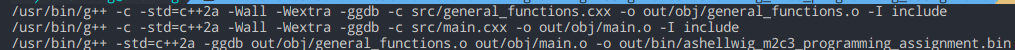
\includegraphics[%
        width={\textwidth}%
      ]{compile.png}
      \caption{Compiling Chapter 4`s Program}
      \label{img:compilation}
    \end{figure}
    \begin{figure}[H]
      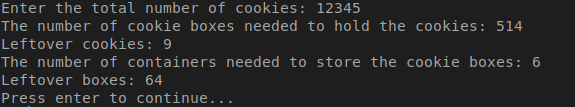
\includegraphics[%
        width={\textwidth}%
      ]{run.png}
      \caption{Running Chapter 4`s Program}
      \label{img:running}
    \end{figure}
    \begin{figure}[H]
      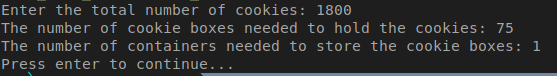
\includegraphics[%
        width={\textwidth}%
      ]{run2.png}
      \caption{Running Chapter 4`s Program -- No leftovers}
      \label{img:running2}
    \end{figure}
\end{document}
